\subsection{بخش ت}
در این بخش به بررسی تفاوت شبیه‌سازی و نتایج مدل در حلقه\LTRfootnote{Model In the Loop(MIL)}
و نرم‌افزار در حلقه\LTRfootnote{Software In the Loop(SIL)} پرداخته شده است. نتایج در ادامه آورده شده است.

\begin{table}[H]
	\caption{ فاصله ازدست‌دهی برای ضریب‌های مختلف تناسبی در قانون هدایت تناسبی حقیقی }
	\centering
	\begin{tabular}{cccc}
		\hline
		 \lr{Miss Distance (m)} &  \lr{Control Effort} & $N'$ & \lr{V-stage}\\
		\hline
		$22.3836$ & $0.8439\!\times\!10^{-8}$ &$3$& \multirow{3}{*}{\lr{MIL}}\\
		$19.6963$ &$0.0834\!\times\!10^{-8}$ &$4$ &\\
		$18.4226$ & $0.9282\!\times\!10^{-8}$  &$5$& \\
		\hline
		$22.3318$ & $0.2691\!\times\!10^{-4}$&$3$ & \multirow{3}{*}{\lr{SIL}}\\
		$19.6759$ &$0.0425\!\times\!10^{-4}$ &$4$&\\
		$18.4123$ & $0.0103\!\times\!10^{-4}$ &$5$& \\
		\hline
	\end{tabular}
\end{table}


\begin{figure}[H]
	\centering
	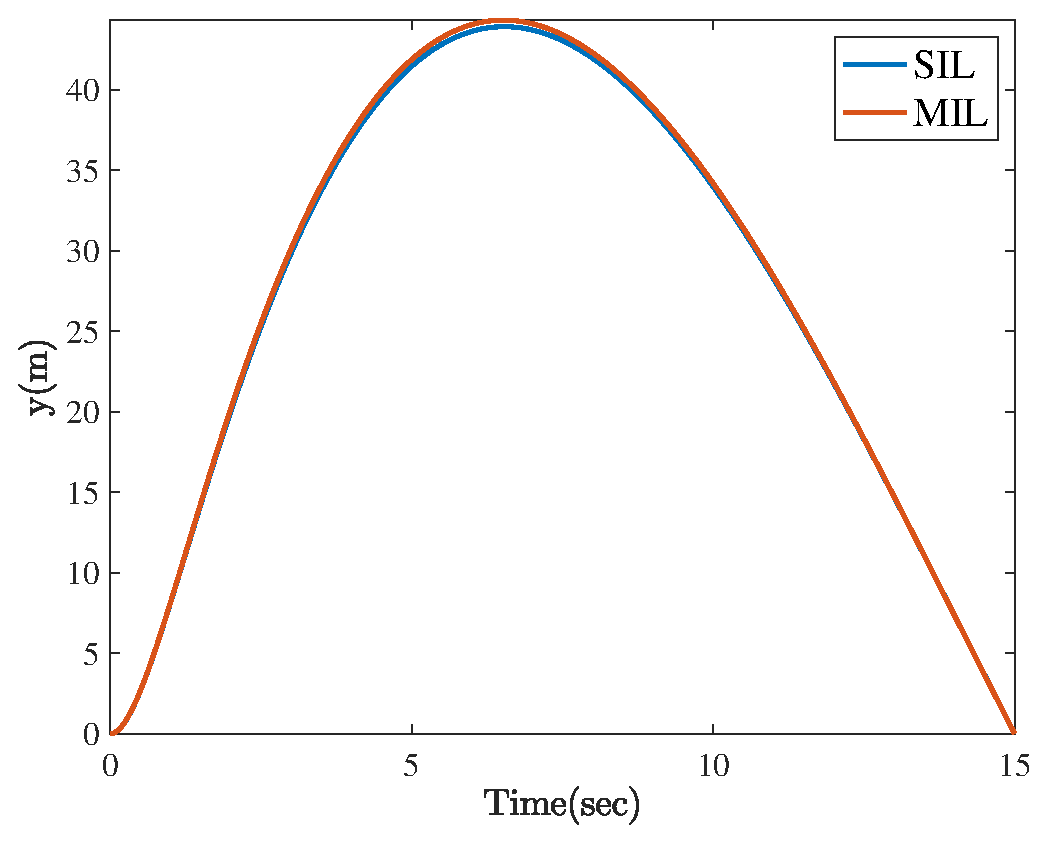
\includegraphics[width=.75\linewidth]{../Figure/Q2/d/y_1}
	\caption{مقایسه نتایج \lr{SIL} و 
		 \lr{MIL}
		 برای متغیر
		\lr{y} 
		در قانون هدایت تناسبی حقیقی برای
	$N'=3$}
\end{figure}

\begin{figure}[H]
	\centering
	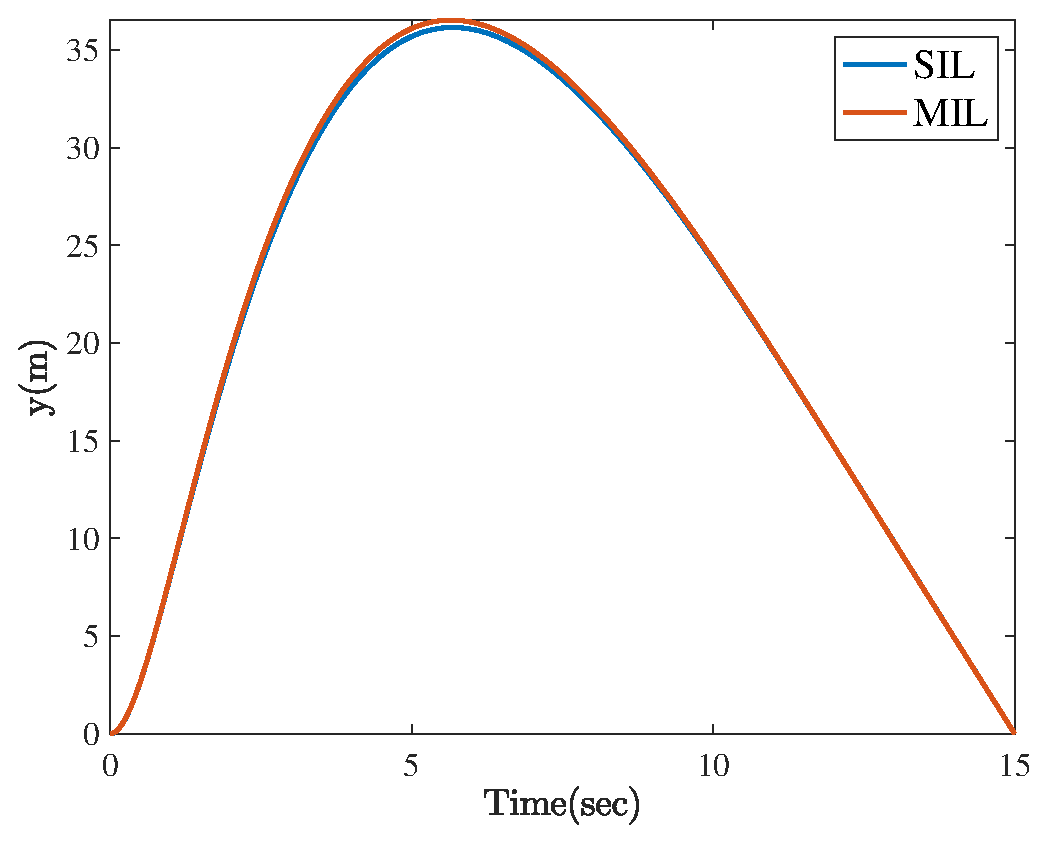
\includegraphics[width=.75\linewidth]{../Figure/Q2/d/y_2}
	\caption{مقایسه نتایج \lr{SIL} و 
		\lr{MIL}
		برای متغیر
		\lr{y} 
		در قانون هدایت تناسبی حقیقی برای
		$N'=4$}
\end{figure}

\begin{figure}[H]
	\centering
	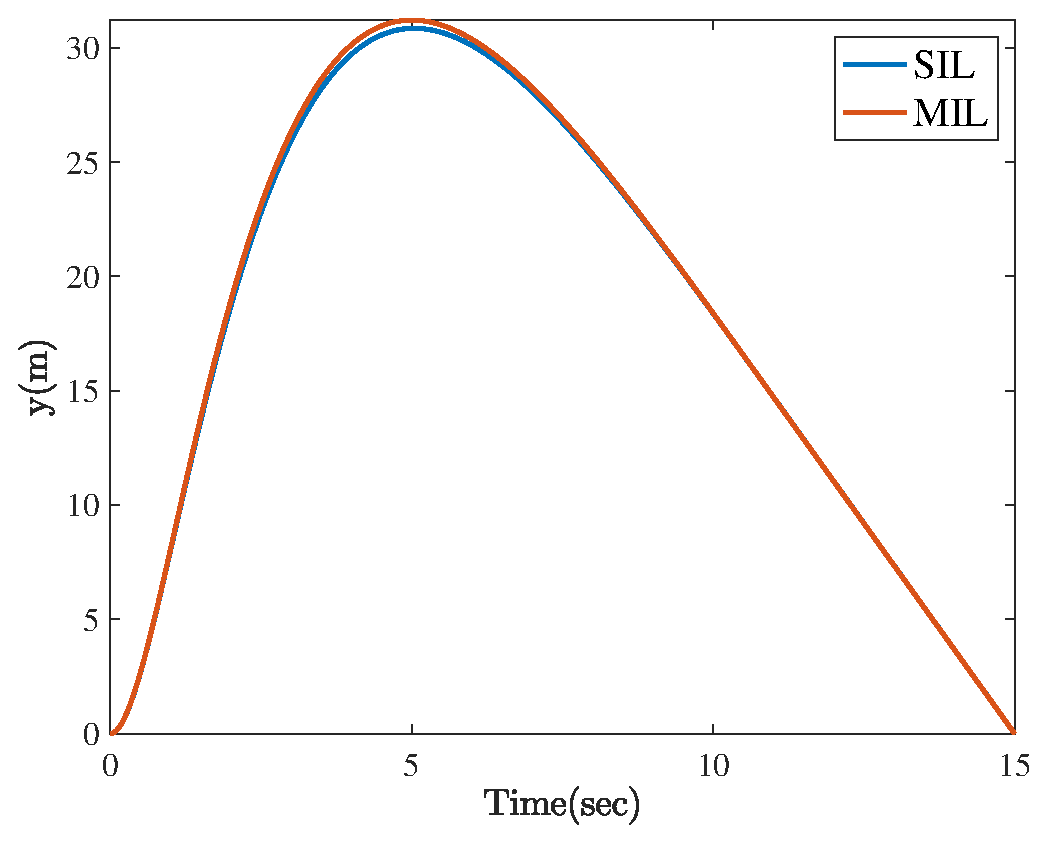
\includegraphics[width=.75\linewidth]{../Figure/Q2/d/y_3}
	\caption{مقایسه نتایج \lr{SIL} و 
		\lr{MIL}
		برای متغیر
		\lr{y} 
		در قانون هدایت تناسبی حقیقی برای
		$N'=5$}
\end{figure}




\begin{figure}[H]
	\centering
	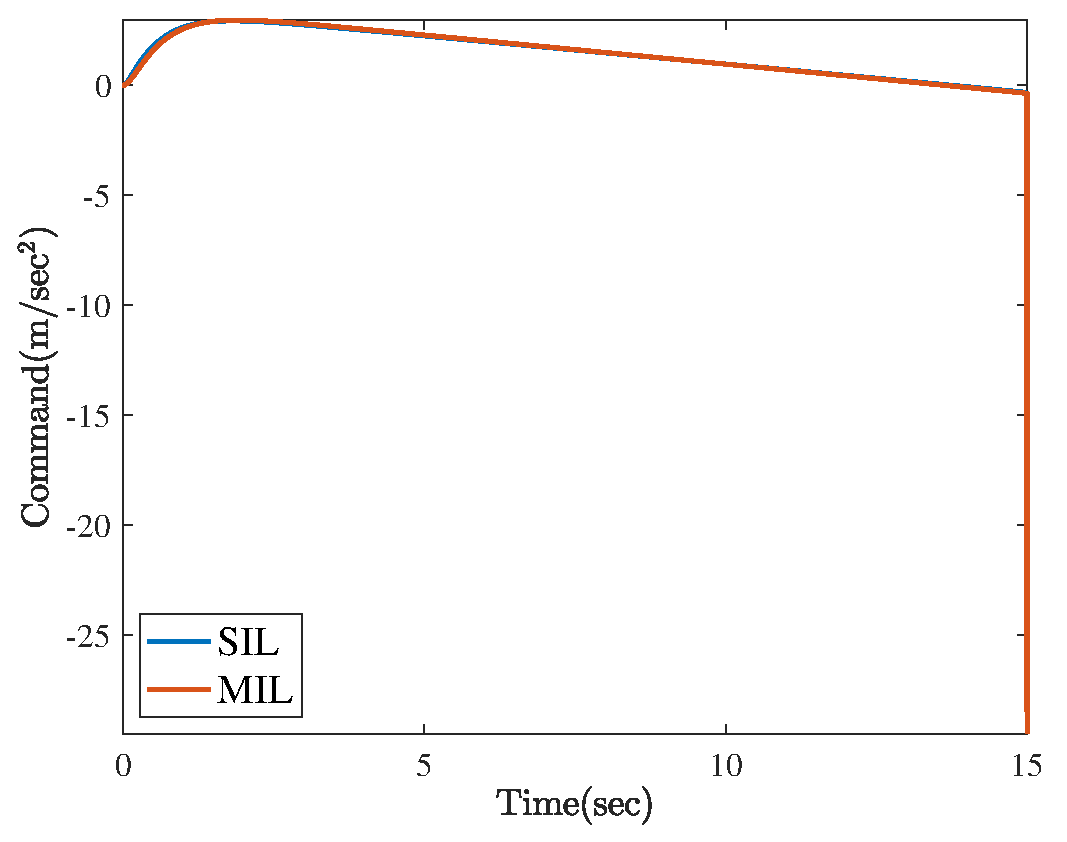
\includegraphics[width=.75\linewidth]{../Figure/Q2/d/command_1}
	\caption{مقایسه تلاش کنترلی \lr{SIL} و 
		\lr{MIL}
		در قانون هدایت تناسبی حقیقی برای
		$N'=3$}
\end{figure}

\begin{figure}[H]
	\centering
	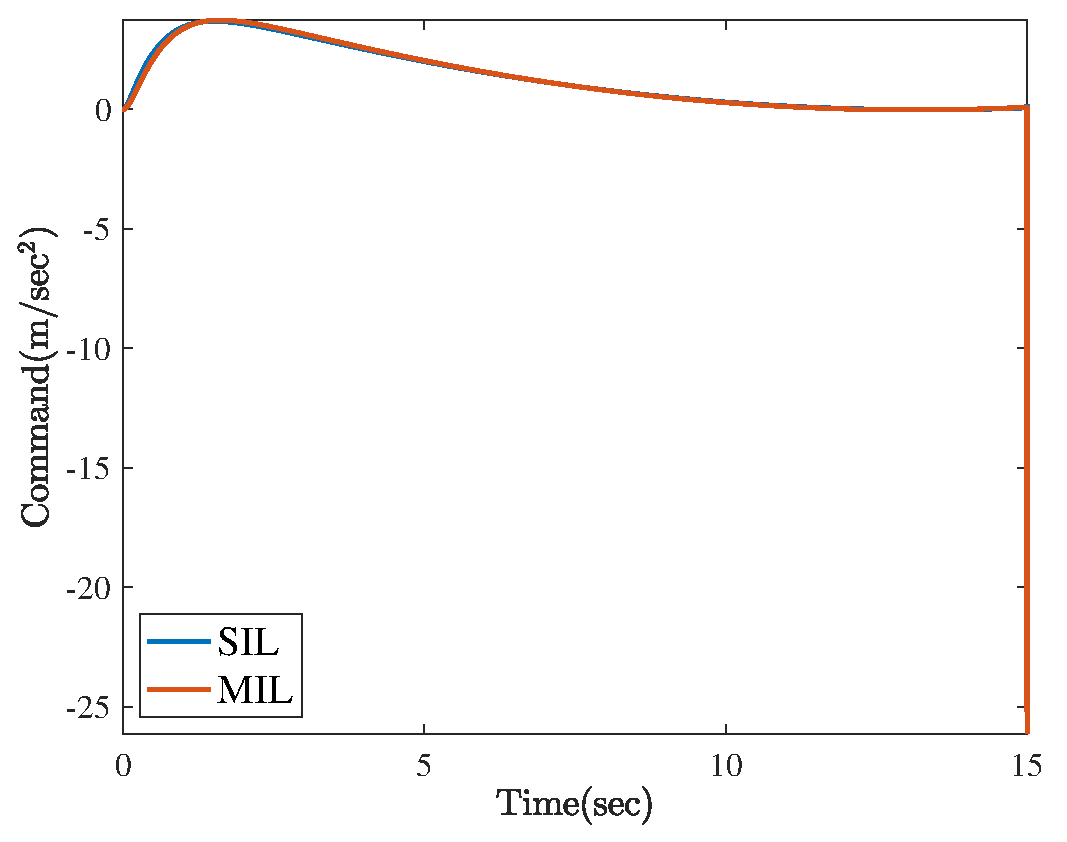
\includegraphics[width=.75\linewidth]{../Figure/Q2/d/command_2}
	\caption{مقایسه تلاش کنترلی \lr{SIL} و 
		\lr{MIL}
		در قانون هدایت تناسبی حقیقی برای
		$N'=4$}
\end{figure}

\begin{figure}[H]
	\centering
	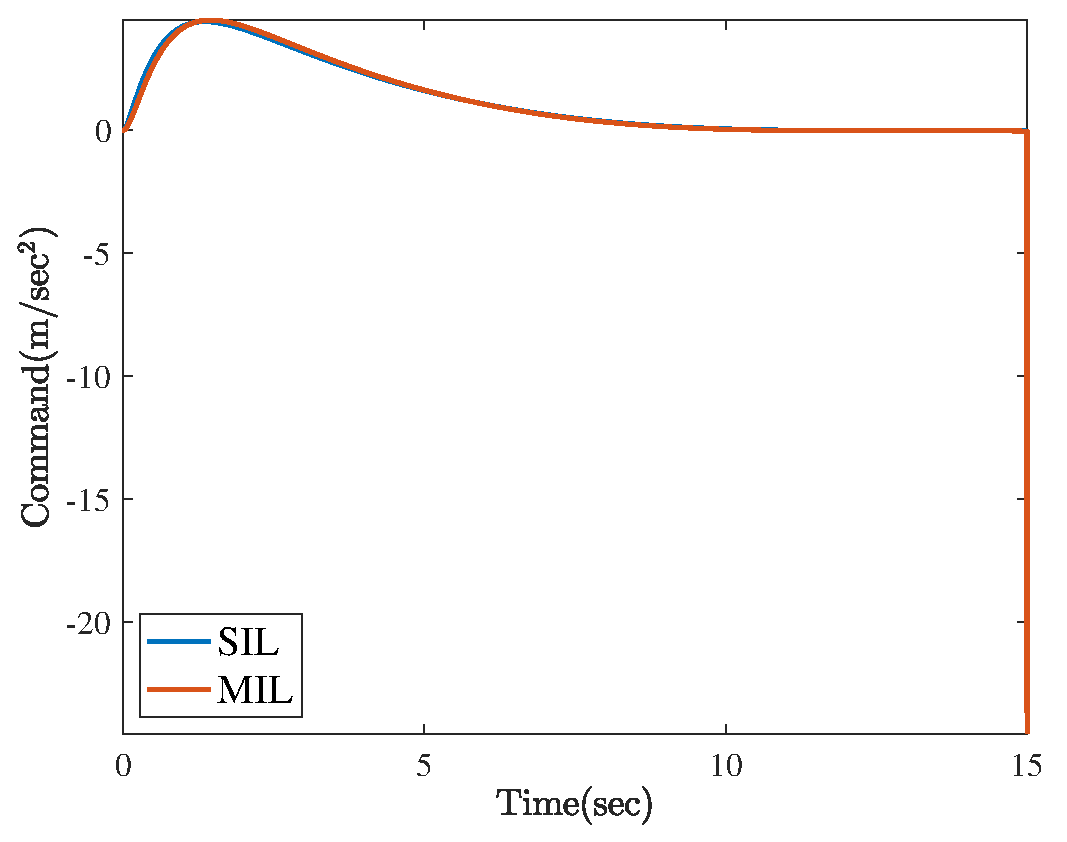
\includegraphics[width=.75\linewidth]{../Figure/Q2/d/command_3}
	\caption{مقایسه تلاش کنترلی \lr{SIL} و 
		\lr{MIL}
		در قانون هدایت تناسبی حقیقی برای
		$N'=5$}
\end{figure}